\documentclass[tikz,border=10pt]{standalone}
\usepackage{tikz}
\usetikzlibrary{shapes,arrows,positioning,fit,backgrounds}

\begin{document}

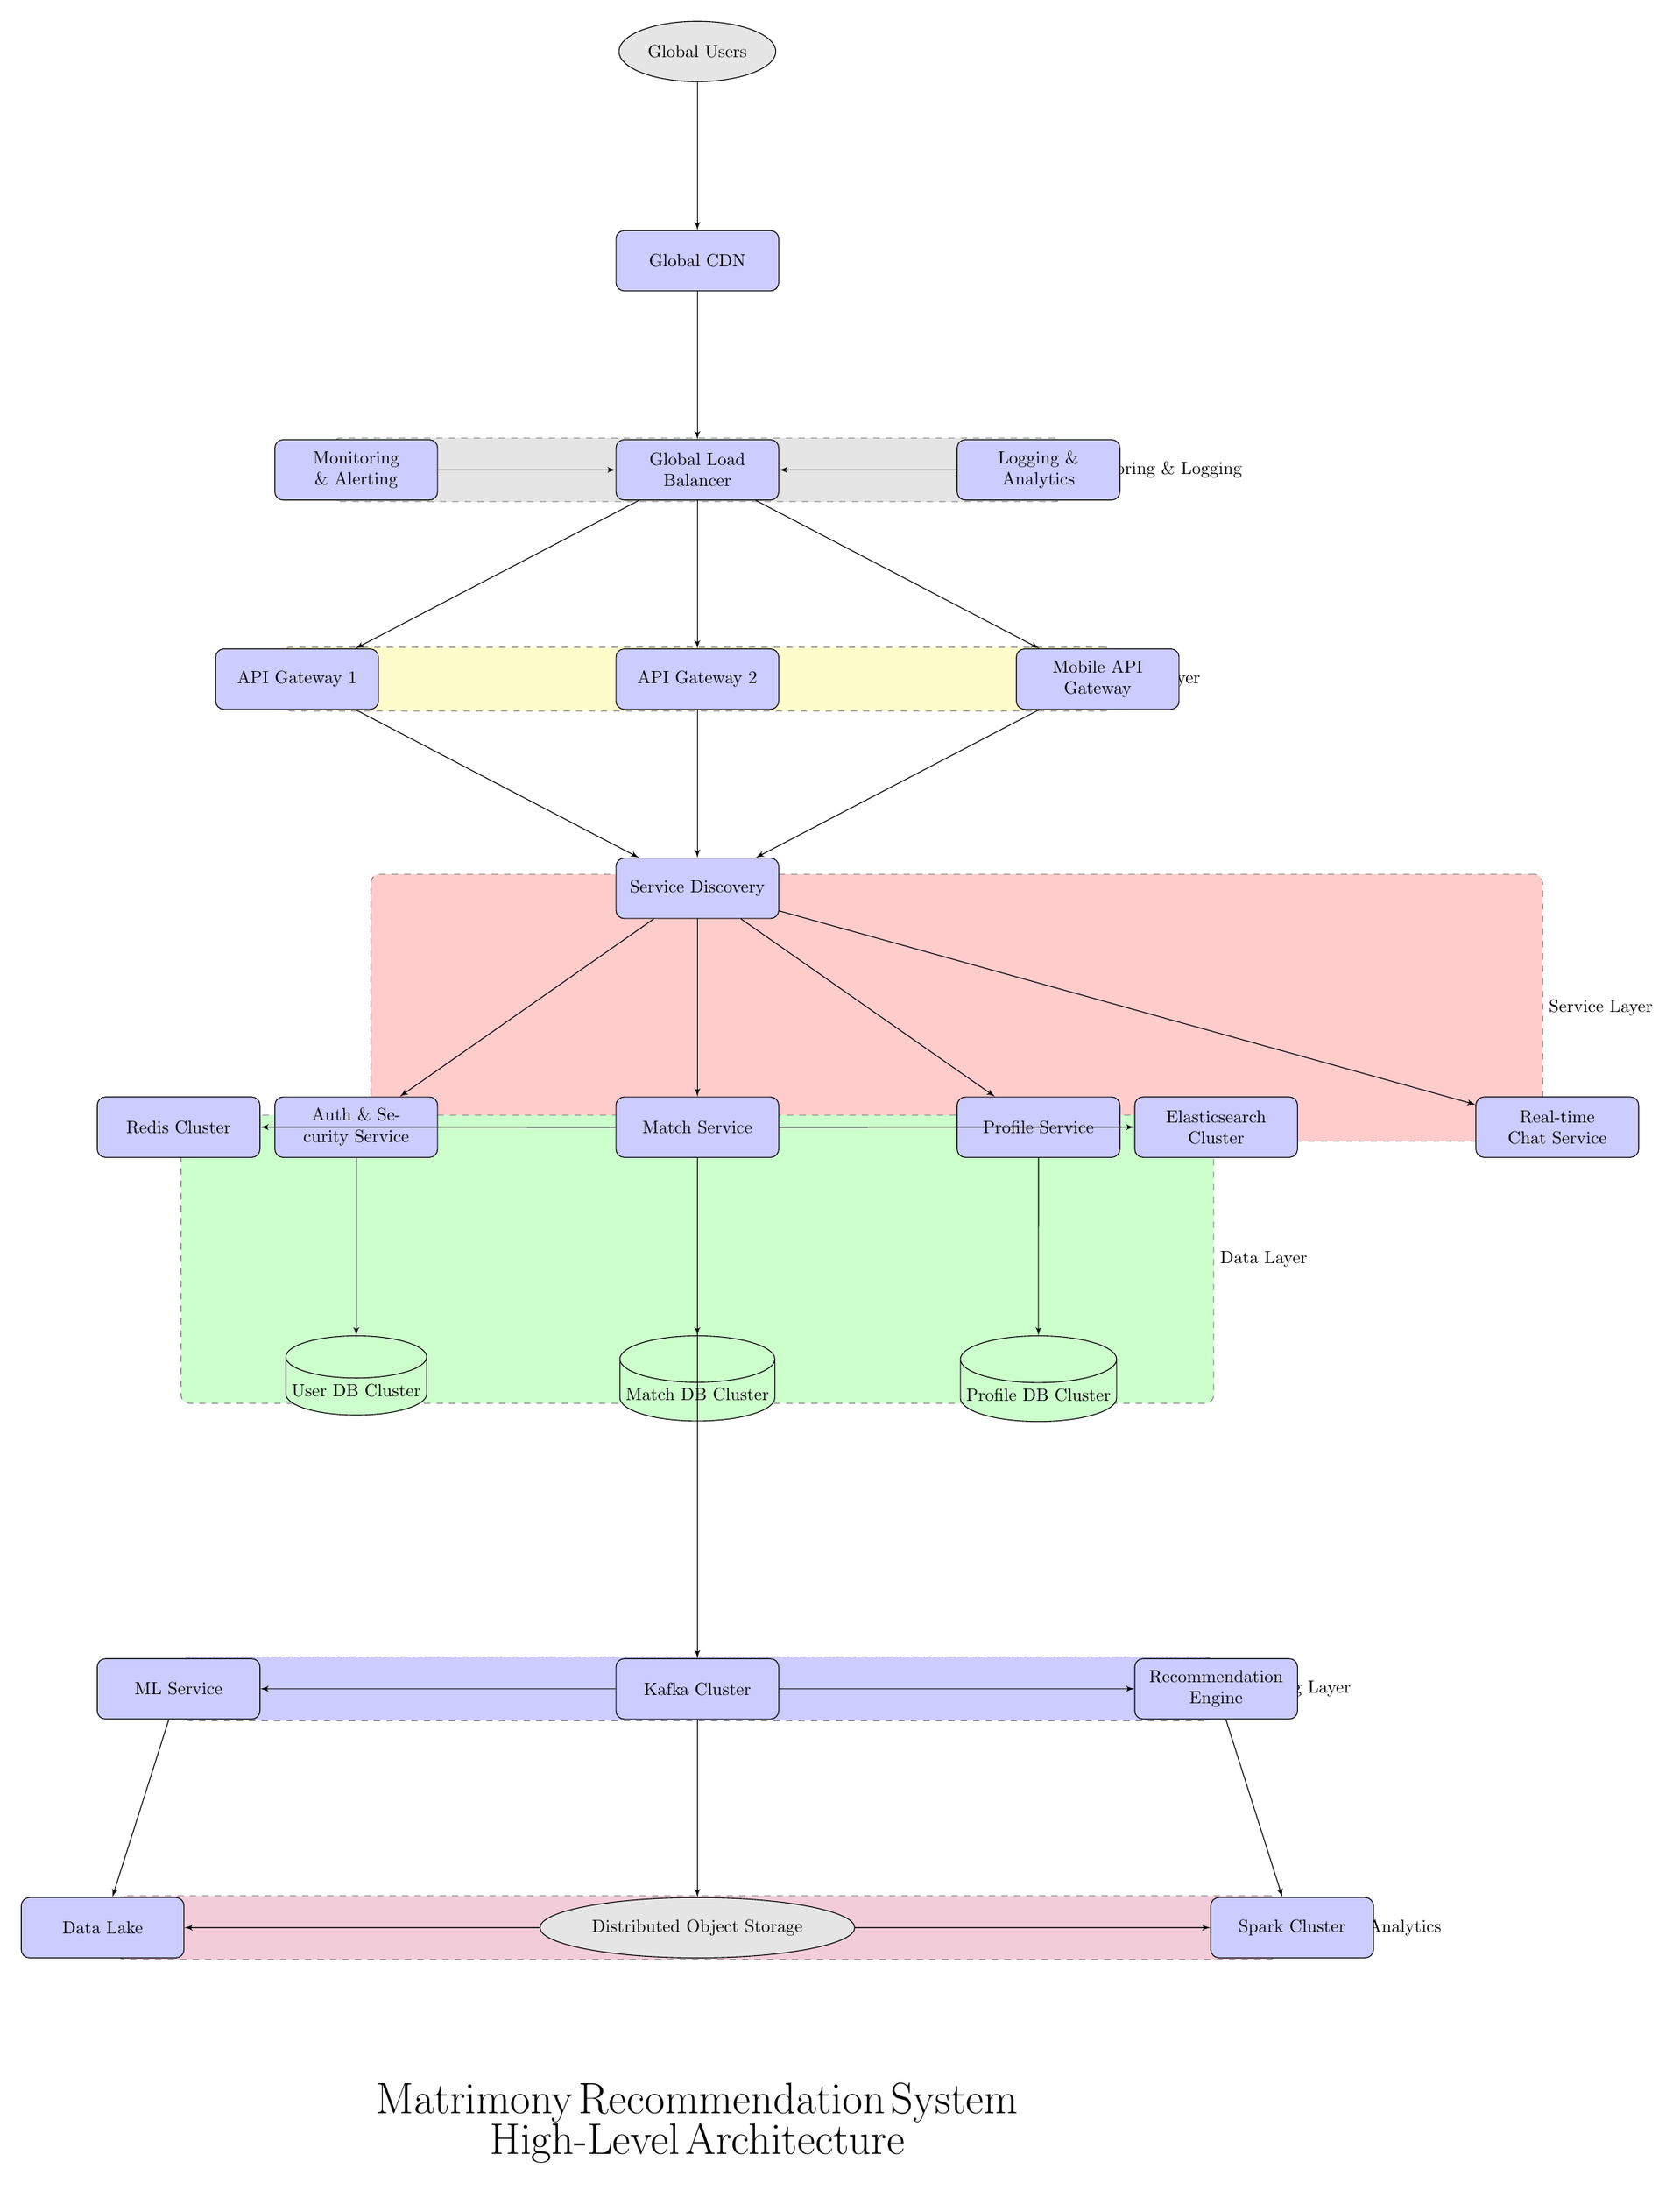
\begin{tikzpicture}[node distance=2.5cm and 4cm, auto, scale=0.85, every node/.style={scale=0.85}]
    % Define styles
    \tikzstyle{component}=[rectangle,rounded corners,draw=black,fill=blue!20,text width=3cm,text centered,minimum height=1.2cm]
    \tikzstyle{database}=[cylinder,draw=black,shape border rotate=90,aspect=0.3,fill=green!20,minimum height=1.2cm,minimum width=1.5cm]
    \tikzstyle{cloud}=[ellipse,draw=black,fill=gray!20,minimum height=1.2cm]
    \tikzstyle{line}=[draw, -latex']

    % Client Layer
    \node [cloud] (users) at (0,0) {Global Users};
    \node [component, below=of users] (cdn) {Global CDN};
    \node [component, below=of cdn] (loadbalancer) {Global Load Balancer};

    % API Gateway Layer
    \node [component, below left=of loadbalancer] (apigateway1) {API Gateway 1};
    \node [component, below=of loadbalancer] (apigateway2) {API Gateway 2};
    \node [component, below right=of loadbalancer] (mobileapigateway) {Mobile API Gateway};

    % Service Layer
    \node [component, below=2.5cm of apigateway2] (servicediscovery) {Service Discovery};
    \node [component, below left=3cm and 3cm of servicediscovery] (authservice) {Auth \& Security Service};
    \node [component, below=3cm of servicediscovery] (matchservice) {Match Service};
    \node [component, below right=3cm and 3cm of servicediscovery] (profileservice) {Profile Service};
    \node [component, right=6cm of profileservice] (chatservice) {Real-time Chat Service};

    % Data Layer
    \node [database, below=3cm of authservice] (userdb) {User DB Cluster};
    \node [database, below=3cm of matchservice] (matchdb) {Match DB Cluster};
    \node [database, below=3cm of profileservice] (profiledb) {Profile DB Cluster};

    % Caching and Search
    \node [component, left=6cm of matchservice] (redis) {Redis Cluster};
    \node [component, right=6cm of matchservice] (elasticsearch) {Elasticsearch Cluster};

    % Messaging and Processing
    \node [component, below=4cm of matchdb] (kafka) {Kafka Cluster};
    \node [component, left=6cm of kafka] (ml) {ML Service};
    \node [component, right=6cm of kafka] (recommendationengine) {Recommendation Engine};

    % Storage and Analytics
    \node [cloud, below=3cm of kafka] (storage) {Distributed Object Storage};
    \node [component, left=6cm of storage] (datalake) {Data Lake};
    \node [component, right=6cm of storage] (spark) {Spark Cluster};

    % Monitoring and Logging
    \node [component, left=3cm of loadbalancer] (monitoring) {Monitoring \& Alerting};
    \node [component, right=3cm of loadbalancer] (logging) {Logging \& Analytics};

    % Define connections
    \path [line] (users) -- (cdn);
    \path [line] (cdn) -- (loadbalancer);
    \path [line] (loadbalancer) -- (apigateway1);
    \path [line] (loadbalancer) -- (apigateway2);
    \path [line] (loadbalancer) -- (mobileapigateway);
    \path [line] (apigateway1) -- (servicediscovery);
    \path [line] (apigateway2) -- (servicediscovery);
    \path [line] (mobileapigateway) -- (servicediscovery);
    \path [line] (servicediscovery) -- (authservice);
    \path [line] (servicediscovery) -- (matchservice);
    \path [line] (servicediscovery) -- (profileservice);
    \path [line] (servicediscovery) -- (chatservice);
    \path [line] (authservice) -- (userdb);
    \path [line] (matchservice) -- (matchdb);
    \path [line] (profileservice) -- (profiledb);
    \path [line] (matchservice) -- (redis);
    \path [line] (matchservice) -- (elasticsearch);
    \path [line] (matchservice) -- (kafka);
    \path [line] (kafka) -- (ml);
    \path [line] (kafka) -- (recommendationengine);
    \path [line] (kafka) -- (storage);
    \path [line] (storage) -- (datalake);
    \path [line] (storage) -- (spark);
    \path [line] (ml) -- (datalake);
    \path [line] (recommendationengine) -- (spark);
    \path [line] (monitoring) -- (loadbalancer);
    \path [line] (logging) -- (loadbalancer);

    % Background rectangles
    \begin{pgfonlayer}{background}
        \node [fill=yellow!20,rounded corners,draw=black!50,dashed,fit=(apigateway1) (apigateway2) (mobileapigateway),label=right:API Layer] {};
        \node [fill=red!20,rounded corners,draw=black!50,dashed,fit=(servicediscovery) (authservice) (matchservice) (profileservice) (chatservice),label=right:Service Layer] {};
        \node [fill=green!20,rounded corners,draw=black!50,dashed,fit=(userdb) (matchdb) (profiledb) (redis) (elasticsearch),label=right:Data Layer] {};
        \node [fill=blue!20,rounded corners,draw=black!50,dashed,fit=(kafka) (ml) (recommendationengine),label=right:Processing Layer] {};
        \node [fill=purple!20,rounded corners,draw=black!50,dashed,fit=(storage) (datalake) (spark),label=right:Storage \& Analytics] {};
        \node [fill=gray!20,rounded corners,draw=black!50,dashed,fit=(monitoring) (logging),label=right:Monitoring \& Logging] {};
    \end{pgfonlayer}

    % Add title
    \node [below=2cm of storage, text width=20cm, align=center] {\Huge Matrimony Recommendation System\\High-Level Architecture};
\end{tikzpicture}

\end{document}
